%\documentclass[a4paper,11pt]{article}

\documentclass[11pt]{report}

% Paquetes comunes
\usepackage[utf8]{inputenc}
\usepackage[spanish]{babel}
\usepackage[T1]{fontenc}
\usepackage{lmodern}
\usepackage{geometry}
\usepackage{setspace}
\usepackage{hyperref}
\usepackage{longtable}
\usepackage{booktabs}
\usepackage{upgreek}
\usepackage{amsmath} 

% Del docs viejo
\usepackage[utf8]{inputenc}
\usepackage[spanish]{babel}
\usepackage[T1]{fontenc}
\usepackage{geometry}
\geometry{a4paper, margin=1in}
\usepackage{graphicx}
\usepackage{subcaption} 
\usepackage{hyperref}
\usepackage{enumitem}
\usepackage{apacite}
\usepackage{natbib}
\usepackage{float}

\geometry{left=3cm,right=3cm,top=3cm,bottom=3cm}
\onehalfspacing


\begin{document}

\begin{titlepage}
    \begin{center}
        
\includegraphics[width=5cm]{Imagenes/Escudo_UBA.png}\\[1cm]

        {\Large \textbf{Universidad de Buenos Aires}}\\[0.2cm]
        \textbf{Facultad de Ciencias Exactas y Naturales}\\[0.2cm]
        \textbf{Maestría en Explotación de Datos y Descubrimiento de Conocimiento}\\[3cm]

        {\Huge \textbf{Proyección de la Calidad del Agua\\
        en el Embalse de Salto Grande}}\\[6cm]

        \textbf\\
        Esp. Joaquín Sebastian Tschopp\\[0.5cm]

        {\normalsize \textbf{Año 2025}}
    \end{center}
\end{titlepage}

%##################################################################################################
%-----------------------------------------------------------------
%  Indice
%-----------------------------------------------------------------


\tableofcontents % presentación Beamer


%##################################################################################################

\newpage

\section*{Resumen}
Este trabajo aborda el desafío de proyectar la calidad del agua en el embalse de Salto Grande, con foco en la playa Las Palmeras, a fin de apoyar decisiones sobre su uso recreativo y tratamiento. Dada la creciente presión sobre los recursos hídricos y la ocurrencia de floraciones de cianobacterias, se buscó anticipar el estado del agua con un horizonte de siete días, integrando datos obtenidos in situ, satelitales, meteorológicos e hidrológicos.

Se aplicaron modelos de aprendizaje automático multiclase, con foco en Random Forest y LightGBM, evaluados mediante validación walk-forward. Se desarrolló un preprocesamiento específico para interpolar variables críticas de baja frecuencia y se diseñó un esquema de cálculo del target basado en los umbrales de la OMS para riesgo sanitario.

Los modelos no lineales entrenados mostraron alto desempeño, alcanzando Random Forest el mejor resultado (F1-score macro de 0{,}9491; exactitud de 0{,}9333) y lograron identificar con alta precisión las clases más críticas. Las variables más relevantes fueron de tipo biológico y fisicoquímico (cianobacterias, clorofila, fósforo total, nitrógeno total), en línea con lo observado en otros estudios sobre el papel de los nutrientes en la aparición de floraciones. El estudio demuestra que es factible integrar modelos predictivos en esquemas de monitoreo operativo, aunque se evidencian limitaciones en la cobertura y frecuencia de los datos que deben ser abordadas en trabajos futuros.

\textbf{Palabras clave:} calidad de agua, cianobacterias, predicción semanal, aprendizaje automático, embalse Salto Grande.

\newpage



%#####################################################################################################



% Capítulo 1: Introducción
\chapter{Introducción}
\section{Contexto y motivación científica}

La calidad del agua es esencial para el consumo humano y para actividades recreativas, especialmente cuando se requiere evaluar la factibilidad de tratamiento y uso del recurso. En un contexto en el que la demanda de recursos hídricos es creciente, determinar la viabilidad de utilizar el agua en el corto plazo resulta crítico para la gestión y la prevención de riesgos.\ref{fig:fauna1} La aplicación de técnicas de Machine Learning, con datos provenientes de diversas fuentes (satelitales, in situ, meteorológicos, hídricos), puede aportar una herramienta de alerta temprana para optimizar la toma de decisiones. La respuesta a esta pregunta contribuirá a la implementación de estrategias de monitoreo y a la mejora en la gestión del recurso hídrico en diferentes puntos del Lago de Salto Grande.

\begin{figure}[h!]
    \centering
    \begin{subfigure}[b]{0.45\textwidth}
        \centering
        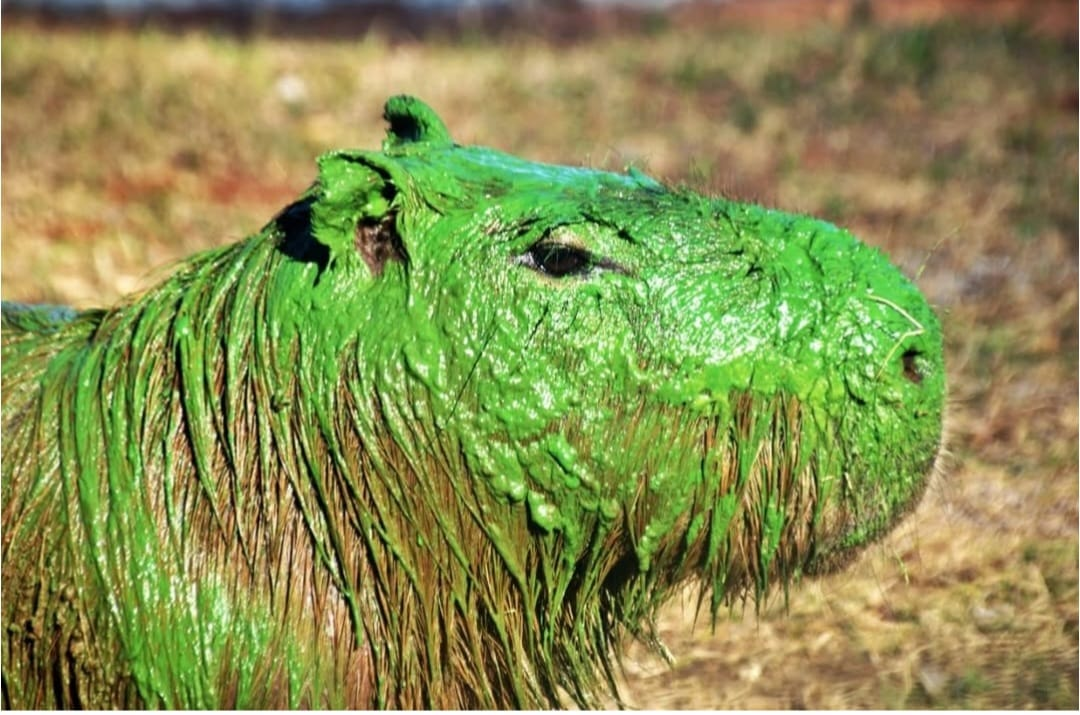
\includegraphics[width=\textwidth]{Imagenes/Fauna_con_Cyano1.jpg}
        \caption{Ejemplo de fauna.}
        \label{fig:fauna1}
    \end{subfigure}
    \hfill
    \begin{subfigure}[b]{0.45\textwidth}
        \centering
        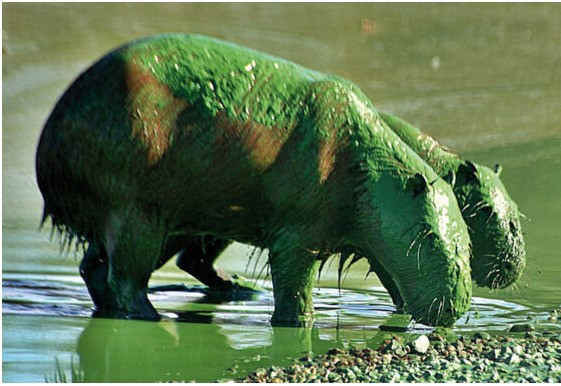
\includegraphics[width=\textwidth]{Imagenes/Fauna_con_Cyano2.jpg}
        \caption{Otro ejemplo de fauna.}
        \label{fig:fauna2}
    \end{subfigure}
    \caption{Imágenes de fauna en áreas con algas. Tomadas por Juan Menoni.}
    \label{fig:fauna}
\end{figure}


\section{Objetivo y Pregunta}

\subsection{Objetivo}
Desarrollar un modelo de proyección semanal que facilite la toma de decisiones acerca del uso del agua en los próximos 7 días (para tratamiento y actividades recreativas como bañarse), integrando información satelital, mediciones in situ, datos meteorológicos e hídricos, y centrando el análisis en la playa \textbf{Las Palmeras}.

\subsection{Pregunta de Investigación}

¿Es factible la proyección del estado de la calidad del agua, basada en las recomendaciones de la Organización Mundial de la Salud para calidad de agua \citep{WHO2021}, en el embalse de Salto Grande, utilizando los datos disponibles y herramientas de predicción de Machine Learning?

\section{Estructura del documento}

El presente trabajo se encuentra organizado en siete capítulos, los cuales abordan de manera progresiva el desarrollo del estudio:

\begin{itemize}
  \item El \textbf{Capítulo 1} introduce el problema de investigación, presenta la motivación científica, define los objetivos del trabajo y describe la organización general del documento.
  
  \item El \textbf{Capítulo 2} recopila y analiza los principales antecedentes y fundamentos teóricos relevantes para el problema abordado. Se describen trabajos previos, marcos normativos y conceptos de ciencia de datos utilizados.
  
  \item El \textbf{Capítulo 3} describe detalladamente la metodología empleada: fuentes y estructura de los datos, técnicas de preprocesamiento, interpolación, definición del objetivo de predicción (\textit{target}), y los modelos de Machine Learning seleccionados, junto con sus criterios de evaluación.
  
  \item El \textbf{Capítulo 4} presenta los resultados obtenidos a partir del entrenamiento y evaluación de los modelos predictivos. Se incluyen análisis comparativos entre algoritmos y se discuten las limitaciones y posibles mejoras del enfoque adoptado.
  
  \item El \textbf{Capítulo 5} resume los principales hallazgos, extrae conclusiones generales en relación con los objetivos planteados y sugiere posibles líneas futuras de investigación o mejora.
  
  \item El \textbf{Capítulo 6} incluye la bibliografía utilizada y citada a lo largo del trabajo, siguiendo el estilo APA.
  
  \item Finalmente, el \textbf{Capítulo 7} incorpora anexos complementarios que contiene referencias al código fuente utilizado en el desarrollo del proyecto.
\end{itemize}


% Capítulo 2: Marco teórico
\chapter{Marco teórico}

\section{Cianobacterias y calidad de agua}

Las cianobacterias son microorganismos fotosintéticos que prosperan en
aguas cálidas y ricas en nutrientes; bajo ciertas condiciones forman
floraciones masivas (\textit{blooms}) capaces de liberar toxinas
nocivas.  Su proliferación depende, sobre todo, de la disponibilidad de
nitrógeno (N) y fósforo (P) y de la estabilidad de la columna de agua.

\paragraph{Factores ambientales.}  
\citep{Igwaran2024} presentan una revisión sistemática de más de 200 investigaciones alrededor del mundo, en el cual identifican los aportes de nitrógeno y fósforo, especialmente provenientes de la agricultura y descargas residuales, como el motor principal de los blooms de cianobacterias, mientras que la temperatura actúa como un factor amplificador, extendiendo la duración de estas proliferaciones.  
De manera análoga,  \citep{Rigosi2014} analizan datos de una extensa evaluación hídrica de más de 1000 lagos en Estados Unidos y concluyen que, en general, los nutrientes tienen un peso mucho mayor que la temperatura en explicar la variación del biovolumen de cianobacterias. Además, su revisión resalta que el estado trófico modula esta relación: los nutrientes dominan en lagos oligotróficos, mientras que el efecto de la temperatura se vuelve relativo en sistemas mesotróficos y eutróficos, donde la interacción nutrientes–temperatura llega a ser relevante.

\paragraph{Implicancias para la salud.}
Las toxinas liberadas (microcistinas, cilindrospermopsina, anatoxinas)
pueden provocar desde irritaciones dérmicas hasta hepatotoxicidad y
fallos neuromusculares.  Un reciente análisis conjunto de casos clínicos
\citep{Backer2024} identifica más de 355 episodios de enfermedad
humana asociados a recreación en aguas contaminadas, destacando que la
inhalación de aerosoles y la ingestión accidental son las vías de
exposición más comunes.

Estos hallazgos sostienen la importancia de vigilar nutrientes,
temperatura y condiciones hidrodinámicas para predecir y mitigar los
blooms, eje central de nuestro modelo de proyección semanal.

\section{Relevamiento de trabajos previos y relevantes}

Diversos estudios han abordado la problemática de la calidad del agua mediante herramientas de aprendizaje automático y observaciones satelitales. \citep{Schaeffer2024}, por ejemplo, presenta una revisión exhaustiva de modelos de predicción aplicados a imágenes de sensores remotos, mostrando el potencial de esta fuente para estimar variables como clorofila-\emph{a}, turbidez y biovolumen de fitoplancton. 

En el estudio de \cite{RodriguezLopez2023}, se evaluó el desempeño de distintos algoritmos de aprendizaje automático para la estimación de parámetros de calidad de agua, en particular clorofila-\emph{a} en el Lago Llanquihue, en el sur de Chile. El trabajo integró 31 años de datos históricos \textit{in situ}, para entrenar modelos con muy buen desempeño, como XGBoost, LightGBM y AdaBoost.

Sin embargo, no todos los trabajos analizados integran datos ambientales correspondientes al momento exacto de las mediciones, ni incorporan variables \textit{in situ} que reflejen condiciones hidrobiológicas o químicas locales. Tampoco se consideran pronósticos meteorológicos de corto plazo como insumo en los modelos predictivos.

\section{Indicadores de riesgo en aguas recreativas}

Los sistemas de alerta para aguas de recreo se basan, por lo general,
en tres indicadores fáciles de medir \citep{WHO2021}:

\begin{itemize}[noitemsep]
  \item \textbf{Concentración de cianobacterias} ($\mathrm{mm^3}/\mathrm{mL}$)
  \item \textbf{Clorofila‑\emph{a}} (µg/L),
  \item \textbf{Transparencia disco Secchi} (m) como indicador turbidez.
\end{itemize}

\paragraph{Muestreo \textit{in situ} vs. teledetección.}
Mientras que el muestreo de campo ofrece precisión puntual, la
teledetección multiplica la cobertura espacial y temporal.
\citep{Stumpf2016} muestran que algoritmos satelitales (MERIS,
actualizados a Sentinel‑3) detectan concentraciones de cianobacterias
con una sensibilidad del 84\%, permitiendo disparar alertas con varios
días de antelación.

\paragraph{Sistemas comparativos.}
\citep{Hunter2022} revisan la implementación de marcos de alerta en
doce países, concluyendo que el esquema OMS de tres niveles es el más
extendido y el que mejor balancea coste–beneficio para la gestión
recreativa en lagos y embalses.

Estos antecedentes sustentan el uso combinado de mediciones
\textit{in situ} y satelitales en nuestro modelo de proyección semanal.

\section{Conceptos y técnicas de ciencia de datos utilizados}

A continuación se describen las principales técnicas de análisis y modelado utilizadas en el desarrollo del presente trabajo, seleccionadas por su adecuación al problema de predicción de alertas semanales de calidad de agua.

\subsection{Interpolación de datos faltantes}

Dado que algunas variables biológicas,  así como métricas hidrológicas claves como el nivel del lago y el aporte del río, presentan baja frecuencia temporal, se aplicaron técnicas de interpolación para completar las series:

\begin{itemize}
  \item \textbf{Interpolación lineal:} útil para aproximar datos entre dos puntos conocidos mediante una recta.
  \item \textbf{Interpolación cúbica (spline):} permite una aproximación más suave entre puntos, conservando continuidad en la primera y segunda derivada.
\end{itemize}

\subsection{Validación y selección de modelos}

Para evitar la fuga de información temporal y asegurar la robustez de los modelos, se utilizó la técnica de validación \textbf{Walk-Forward} tanto para la validación durante la búsqueda de hiperparámetros como para la evaluación en test.

\subsection{Modelos supervisados multiclase}

Se compararon cuatro algoritmos de clasificación con diferentes capacidades y supuestos:

\begin{itemize}
  \item \textbf{Regresión logística multinomial:} modelo lineal base.
  \item \textbf{Máquinas de soporte vectorial (MSV):} clasificador no lineal.
  \item \textbf{Random Forest:} ensamble de árboles, robusto a ruido y capaz de capturar interacciones.
  \item \textbf{LightGBM:} algoritmo de boosting eficiente y escalable.
\end{itemize}


% Capítulo 3: Metodología
\chapter{Metodología}
\section{Presentación y descripción de los datos utilizados}
%-----------------------------------------------------------------
%  Conjunto de Datos
%-----------------------------------------------------------------
\subsection{Conjunto de Datos}

\subsubsection{Fuentes de obtención}
\begin{itemize}[noitemsep]
    \item \textbf{Comisión Técnica Mixta de Salto Grande:} Datos \textit{in situ} (mediciones directas en el lugar de estudio y resultados de laboratorio de muestras tomadas en ese sitio), junto con registros hidrometeorológicos.
    \item \textbf{Imágenes satelitales:} Sentinel-2 y Landsat 8/9.\ref{fig:cyano_en_lago}
    \item \textbf{Estaciones meteorológicas:} Lluvia, temperatura, viento.
    \item \textbf{Modelos meteorológicos:} Pronóstico de precipitaciones y temperatura, a 1–6 días.
\end{itemize}

\begin{figure}[h!]
    \centering
    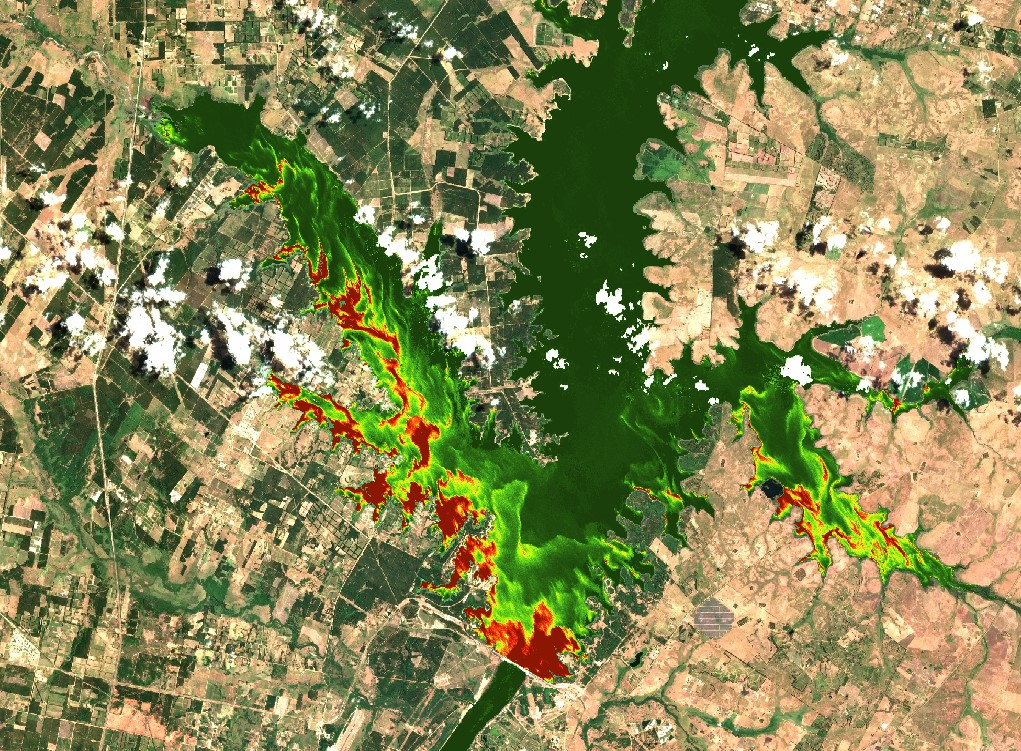
\includegraphics[width=0.6\textwidth]{Imagenes/Cyano_en_lago.jpg}
    \caption{Imagen satelital que muestra la presencia de cianobacterias en el embalse. Las zonas en rojo indican áreas con alta concentración de floraciones (\textit{blooms}).}
    \label{fig:cyano_en_lago}
\end{figure}

\subsubsection{Estructura de los datos}

A continuación se describen brevemente los atributos del dataset, sus tipos de dato y su significado.

\begin{longtable}{llp{8cm}}
\caption{Descripción de los atributos y sus tipos en el dataset.} \label{tab:estructura-datos} \\
\hline
\textbf{Atributo} & \textbf{Tipo} & \textbf{Descripción} \\
\hline
\endfirsthead

\hline
\textbf{Atributo} & \textbf{Tipo} & \textbf{Descripción} \\
\hline
\endhead

\hline
\multicolumn{3}{r}{\emph{Continúa en la siguiente página}} \\
\endfoot

\hline
\endlastfoot

time & \texttt{datetime} & Identificación del registro (fecha y hora) \\
T.obs & \texttt{float64} & Temp. media observada (se toma la media) \\
Hr.obs & \texttt{float64} & Humedad relativa (media) \\
pr.obs & \texttt{float64} & Presión atmosférica (media) \\
Rad.obs & \texttt{float64} & Radiación solar (media) \\
u.obs & \texttt{float64} & Velocidad del viento (media) \\
u\_gr.obs & \texttt{float64} & Dirección del viento (grados: 0=Norte, 90=Este, 180=Sur, 270=Oeste) \\
Td.obs & \texttt{float64} & Temperatura de punto de rocío \\
EPenman.obs & \texttt{float64} & Evapotranspiración (método Penman) \\
pp\_obs & \texttt{float64} & Precipitación observada diaria (mm) \\
\hline
\multicolumn{3}{l}{\textbf{Pronóstico meteorológico}} \\
prono\_PP\_dia\_[0–6] & \texttt{float64} & Pronóstico de precipitación diaria (mm) \\
prono\_Tm\_dia\_[0–7] & \texttt{float64} & Pronóstico de temperatura media diaria (°C) \\
\hline
Cianorg & \texttt{float64} & Cianobacterias totales (org/mL) \\
Clorof\_A & \texttt{float64} & Concentración de clorofila-a (\(\mu\)g/L) \\
Enteroc & \texttt{float64} & Recuento de enterococos (NMP/100 mL) \\
NO2\_lab & \texttt{float64} & Nitrito (mg/L) \\
NO3\_lab & \texttt{float64} & Nitrato (mg/L) \\
NT & \texttt{float64} & Nitrógeno total (mg/L) \\
Ptot\_lab & \texttt{float64} & Fósforo total (mg/L) \\
\hline
SS\_105 & \texttt{float64} & Sólidos suspendidos medidos a 105°C (mg/L) \\
ODsupC & \texttt{float64} & Oxígeno disuelto en superficie corregido (mg/L) \\
TempAmb & \texttt{float64} & Temperatura ambiente (°C) \\
TurSupC & \texttt{float64} & Turbidez en superficie corregida (NTU) \\
PO4\_lab & \texttt{float64} & Fosfato reactivo medido en laboratorio (mg/L) \\
SS\_550 & \texttt{float64} & Sólidos suspendidos medidos a 550°C (mg/L) \\
NH\_lab & \texttt{float64} & Amonio medido en laboratorio (mg/L) \\
MCys\_spp & \texttt{float64} & Abundancia de Microcystis spp. (org/mL) \\
VientoI & \texttt{float64} & Intensidad del viento (km/h) \\
Cianobac & \texttt{float64} & Recuento total de cianobacterias (org/mL) \\
T\_sup & \texttt{float64} & Temperatura del agua en superficie (°C) \\
CondsupC & \texttt{float64} & Conductividad eléctrica sup. corregida (µS/cm) \\
MicrtEli & \texttt{float64} & Microtendipes y Elissoma (org/mL) \\
EscColi & \texttt{float64} & Recuento de Escherichia coli (NMP/100 mL) \\
PROFSITI & \texttt{float64} & Profundidad de sitio de muestreo (m) \\
SatSupC & \texttt{float64} & Saturación de oxígeno en sup. corregida (\%) \\
fitotot & \texttt{float64} & Biomasa total de fitoplancton (µg/L) \\
pHsupC & \texttt{float64} & pH en superficie corregido (adimensional) \\
Secc\_sup & \texttt{float64} & Profundidad Secchi en superficie (m) \\
Nivel\_lago & \texttt{float64} & Nivel del embalse (m) \\
Caudal\_lago & \texttt{float64} & Caudal de aporte (m³/s) \\
Target & \texttt{float64} & Nivel de alerta OMS: 0=Sin Riesgo, 1=Vigilancia, 2=Alerta 1, 3=Alerta 2 \\
\end{longtable}

\section{Preprocesamiento y limpieza de los datos}

%-------------------------------------------------------------
\subsection{Aumentación por interpolación}
%-------------------------------------------------------------

El conjunto de datos utilizado presenta frecuencias dispares según el tipo de variable. Para poder entrenar modelos de aprendizaje automático con entradas diarias consistentes, fue necesario completar ciertas series temporales mediante técnicas de interpolación, preservando al mismo tiempo la estructura original de la información. A continuación se detallan los métodos aplicados según la naturaleza de los datos.

%-------------------------------------------------------------
\subsubsection{Interpolación funcional en variables biológicas}
%-------------------------------------------------------------

Las variables biológicas claves (biovolumen de cianobacterias, clorofila-\textit{a}, fitoplancton total, etc.) fueron medidas con baja frecuencia (una vez por semana en verano y una vez al mes en invierno), lo que imposibilita un entrenamiento robusto. Para resolver esta limitación, se aplicó una estrategia de interpolación funcional basada en el trabajo de \citep{Oh2020}, con el siguiente procedimiento:


\begin{enumerate}[noitemsep]
  \item \textbf{Segmentación temporal}\,: la serie se divide en ventanas fijas.
  \item \textbf{Ajuste de funciones suaves}\,: en cada ventana se ajusta una spline cúbica natural que minimiza la curvatura entre puntos reales, forzando a que la curva pase exactamente por los valores observados.
  \item \textbf{Muestreo denso}\,: la spline se evalúa a paso diario, generando valores sintéticos que respetan la tendencia local y preservan continuidad.
  \item \textbf{Unión de ventanas}\,: se superponen días en los bordes para garantizar suavidad entre segmentos.
  \item \textbf{Truncamiento de valores}\,: al finalizar el proceso, los valores generados que exceden el máximo observado o descienden por debajo de cero son truncados, evitando así la aparición de outliers superiores a los reales y de valores negativos artificiales.
\end{enumerate}

El resultado es una serie diaria suave que conserva la forma global del fenómeno observado, introduce variación controlada útil para el aprendizaje supervisado, y garantiza que los valores sintéticos sean físicamente plausibles.


%-------------------------------------------------------------
\subsubsection{Interpolación lineal en variables hidrológicas}
%-------------------------------------------------------------

Las variables hidrológicas, \texttt{Nivel\_lago} y \texttt{Caudal\_lago}, se encuentran disponibles con frecuencia semanal, representando valores promedio. Para completar las fechas intermedias entre mediciones y armonizar la frecuencia con el resto del dataset, se aplicó interpolación lineal entre puntos consecutivos, siguiendo la implementación disponible en \texttt{scipy.interpolate} \citep{virtanen2020scipy}.

Dado que los valores originales ya representan medias semanales, la interpolación lineal entre ellos resulta una estrategia adecuada para generar estimaciones coherentes.


%-------------------------------------------------------------
\subsection{Cálculo del \textit{target}}
%-------------------------------------------------------------
Los umbrales se toman de la OMS \citep{WHO2021}, ajustados a las
variables disponibles en nuestro registro (no se tuvieron en cuenta las mediciones de toxinas).

\begin{itemize}[leftmargin=*]
  \item \textbf{Sin Riesgo (0)}
        \begin{itemize}[noitemsep]
            \item Biovolumen $\leq 1\,\mathrm{mm}^3/\mathrm{L}$, \textbf{o}
            \item Clorofila-\emph{a} $\leq 3\,\upmu\mathrm{g}/\mathrm{L}$ con dominancia de cianobacterias, \textbf{o}
            \item Transparencia Secchi $> 2$ m.
        \end{itemize}

        
  \item \textbf{Vigilancia (1)}
        \begin{itemize}[noitemsep]
          \item Biovolumen $\in [1,\ 4]$\,mm$^{3}$/L, \textbf{o}
          \item Clorofila‑\emph{a} $\in [3,\ 12]$\,$\upmu$ug/L con dominancia de cianobacterias, \textbf{o}
          \item Transparencia Secchi $\in [1,\ 2]$\,m.
        \end{itemize}

  \item \textbf{Alerta1 (2)}
        \begin{itemize}[noitemsep]
          \item Biovolumen $\in [4,\ 8] $\,mm$^{3}$/L, \textbf{o}
          \item Clorofila‑\emph{a} $\in [12,\ 24] $\,$\upmu$ug/L con dominancia de cianobacterias, \textbf{o}
          \item Transparencia Secchi $\in [0.5,\ 1] $\,m.
        \end{itemize}

  \item \textbf{Alerta2 (3)}
        \begin{itemize}[noitemsep]
          \item Presencia de \emph{scum} de cianobacterias \textbf{o}
          \item Clorofila‑\emph{a} $> 24$\,$\upmu$ug/L, \textbf{o}
          \item Transparencia Secchi $< 0.5$\,m.
        \end{itemize}
\end{itemize}

\textbf{Conversión de unidades mediante regresión lineal.}  
La variable correspondiente a la cianobacteria fue transformada a mm$^{3}$/L utilizando un modelo de regresión lineal entrenado con datos de años en que se registraron ambas magnitudes. La ecuación resultante fue:

\[
\text{BVCIANsp} = 0{,}0001 \times \text{Cianobac} + 0{,}2006
\]

El modelo obtuvo los siguientes índices:

\begin{itemize}[noitemsep]
  \item Coeficiente de determinación: $R^2 = 0{,}994$
  \item Error cuadrático medio (RMSE): $0{,}4720$
\end{itemize}

Estos resultados (LinearRegression(): $R^2 = 0{,}9942645$, RMSE = $0{,}472014$) indican que se trata de un estimador muy preciso. La decisión de emplearlo fue tomada conjuntamente con el personal encargado de la recolección de muestras y de la interpretación de los atributos.

Esta transformación garantiza la compatibilidad de las unidades derivadas con los umbrales de la OMS para biovolumen de cianobacterias (mm$^{3}$/L) y preserva la calidad interpretativa de los datos.

\textbf{Asignación del target a futuro.} 
Para modelar la predicción de la calidad del agua con una anticipación de 7 días, se asignó a cada registro el valor del target correspondiente a 7 días después. Así, al entrenar el modelo con los datos disponibles hasta una fecha determinada, se busca predecir el estado de la calidad del agua una semana más adelante \citep{datacamp2022forecasting}. Por ejemplo, si se realiza una predicción utilizando los datos del 01-01-2025, el modelo estará estimando el estado correspondiente al 08-01-2025. Esta estrategia permite que el modelo aprenda a anticipar condiciones futuras basándose únicamente en información pasada, respetando la secuencia temporal de los datos.


Sin embargo, debido a la frecuencia irregular de las observaciones reales, no fue posible construir un target uniforme con un horizonte fijo de 7 días sin recurrir a interpolación. En muchos casos, la distancia entre una observación y la siguiente superaba los 7 días (por ejemplo, 10 o 30 días), lo que impedía definir con precisión el estado futuro deseado. Esta situación hacía inviable el entrenamiento del modelo exclusivamente con datos reales, ya que se perdería una porción sustancial del conjunto de entrenamiento. Por este motivo, se optó por aplicar interpolaciones controladas para completar la secuencia temporal y permitir la construcción de un target coherente, aún reconociendo los riesgos que esto implica en términos de sobreajuste y fidelidad de los patrones aprendidos.


\subsection{Filtrado de registros con datos faltantes}

Durante el preprocesamiento de los datos, se eliminaron los registros iniciales y finales que presentaban valores faltantes en las variables hidrológicas, meteorológicas y biológicas. Esta decisión se tomó para asegurar que los conjuntos de entrenamiento y prueba contuvieran únicamente datos reales de calidad del agua, evitando así la influencia de valores interpolados en los extremos de la serie temporal.


%##############################################################################################

\section{Análisis exploratorio de datos (EDA)}

Se realizó un EDA agrupando las variables por su naturaleza.

\subsection{Resumen estadístico por grupo}

Se analizó la distribución básica de los valores por grupo de variables. A continuación se resumen los principales hallazgos:

\paragraph{Variables meteorológicas.}
Las temperaturas observadas (\texttt{T.obs}) presentan una media de 20.2°C, con un rango que va de 5.8 a 34.3°C. La humedad relativa (\texttt{Hr.obs}) tiene una amplia dispersión, con valores entre 34\% y casi 100\%. La radiación solar (\texttt{Rad.obs}) y la presión atmosférica (\texttt{pr.obs}) exhiben también alta variabilidad. Se observa una anomalía en \texttt{u.obs} (velocidad del viento) con un valor mínimo de –1039, lo que sugiere posibles errores de medición o registro.Los valores negativos detectados en esta variable fueron corregidos a cero para evitar distorsiones en el análisis.

\paragraph{Variables hidrológicas.}
El caudal de aporte (\texttt{Aporte\_m3s}) muestra alta dispersión (std $\approx$ 4884), con valores que oscilan entre 410 y más de 25000 m³/s. El nivel del embalse (\texttt{Nivel\_emb}) oscila entre 30.87 y 35.42 m, con media de 33.7m.

\paragraph{Variables biológicas.}
Las variables biológicas como \texttt{Cianorg} y \texttt{Clorof\_A} presentan fuerte asimetría. Por ejemplo, \texttt{Clorof\_A} varía entre 0.3 y más de 1250 µg/L (media: 52.2), mientras que \texttt{Cianobac} tiene una media de 75,934 org/mL y un máximo superior a 2.4 millones.

\paragraph{Variables químicas.}
El nitrógeno total (\texttt{NT}) y el fósforo total (\texttt{Ptot\_lab}) presentan valores dentro de rangos esperados, pero con leve sesgo positivo. La variable \texttt{SS\_105} también muestra dispersión significativa (hasta 42.7 mg/L).

\paragraph{Otras variables.}
La conductividad eléctrica en superficie (\texttt{CondsupC}) presenta alta variabilidad (hasta 1575 µS/cm). La temperatura ambiente (\texttt{TempAmb}) oscila entre 13 y 35°C, mientras que el viento (\texttt{VientoI}) alcanza máximos de 24km/h.

En todos los grupos se observaron valores extremos (outliers) y distribuciones sesgadas, lo que motiva el uso de transformaciones, normalización y modelos robustos para el análisis posterior.

\subsection{Distribuciones y valores atípicos}

Se analizaron las distribuciones de seis variables relevantes, en función del nivel de alerta definido por la OMS y de trabajos de investigación que resaltan su importancia. En la Figura~\ref{fig:outliers-boxplots} se presentan boxplots para cada variable, lo que permite identificar diferencias entre las clases del target y observar la presencia de valores extremos.

La variable \texttt{Clorof\_A} presenta una marcada asimetría positiva, con valores atípicos más frecuentes en el nivel de alerta 0 y 1. Asimismo, las variables \texttt{SS\_105}, \texttt{SS\_550}, \texttt{Ptot\_lab}, \texttt{PO4\_lab} y \texttt{NO2\_lab} muestran variaciones significativas en sus distribuciones entre clases, evidenciadas por el incremento de la mediana y del rango superior en los estados más críticos.

\begin{figure}[H]
    \centering
    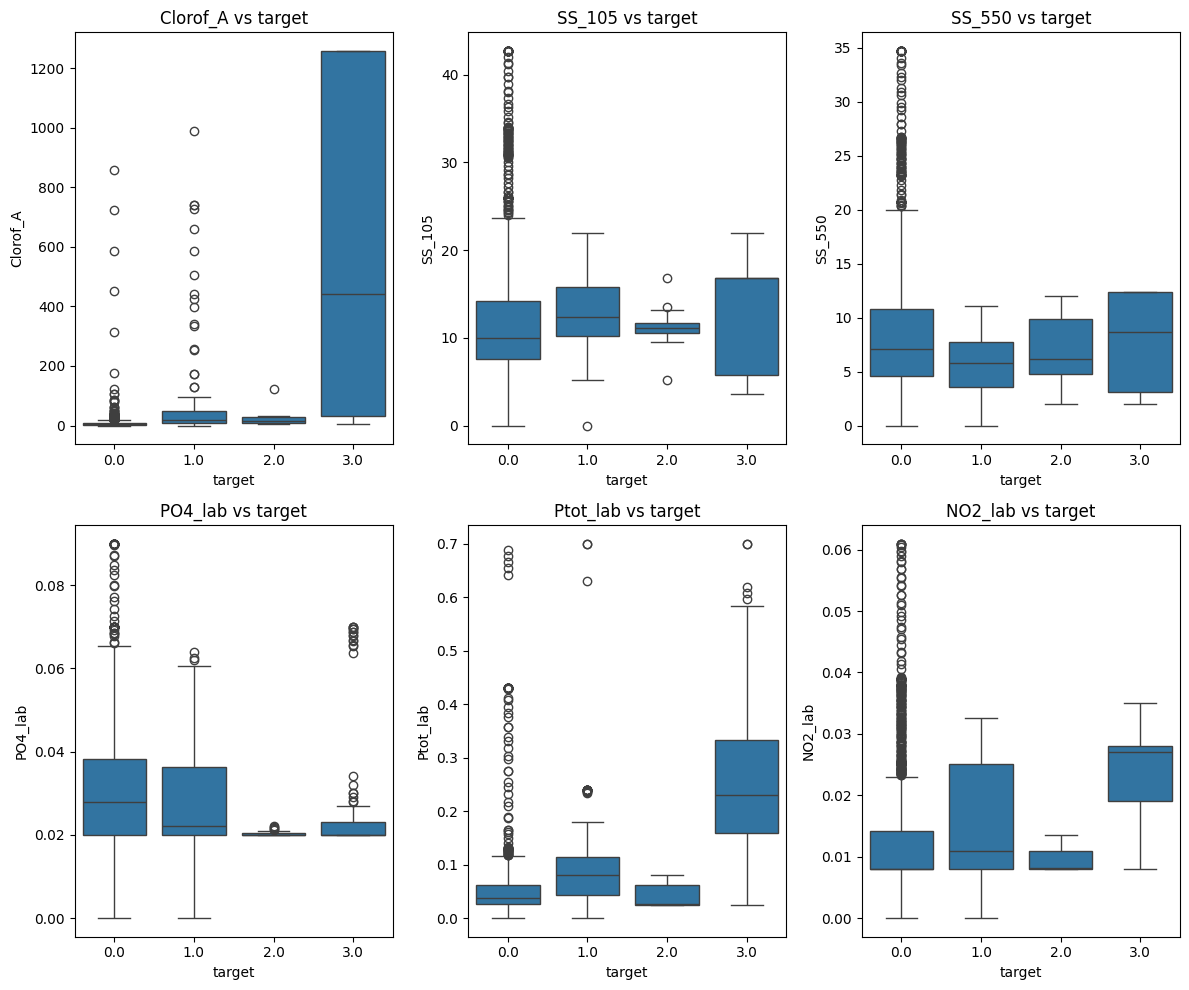
\includegraphics[width=0.95\textwidth]{Imagenes/Boxplots_Target_3x2.png}
    \caption{Distribución de variables seleccionadas respecto al nivel de alerta. Se observa presencia de valores atípicos en múltiples clases, especialmente en el nivel 0.}
    \label{fig:outliers-boxplots}
\end{figure}

\subsection{Correlaciones entre variables}

Se construyó una matriz de correlación de Pearson entre todas las variables numéricas del conjunto de datos, limitada a coeficientes de correlación mayores a 0.5 para facilitar la lectura (ver Figura~\ref{fig:correlaciones}).

Se observan altas correlaciones entre variables relacionadas con sólidos en suspensión (\texttt{SS\_105} y \texttt{SS\_550}), y entre estas y \texttt{Aporte\_m3s} y \texttt{EnterocPO4\_lab} aunque mas leve. Además, las variables de temperatura muestran cierta correlación con la radiación y la conductividad. Estas relaciones sugieren que existen grupos de variables que responden a procesos ambientales similares o diferentes formas de medir atributos similares, lo que puede ser relevante al momento de seleccionar variables para los modelos predictivos y evitar problemas de multicolinealidad.

Se observan altas correlaciones entre variables relacionadas con sólidos en suspensión (\texttt{SS\_105} y \texttt{SS\_550}), y entre estas y \texttt{Aporte\_m3s}; también se identifica correlación moderada con \texttt{Enteroc}. Además, las variables de temperatura muestran cierta correlación con la radiación y la conductividad. Estas relaciones sugieren que existen grupos de variables que responden a procesos ambientales similares, o bien distintas formas de medir atributos relacionados, lo que puede ser relevante al momento de seleccionar variables para los modelos predictivos y evitar problemas de multicolinealidad.


\begin{figure}[H]
    \centering
    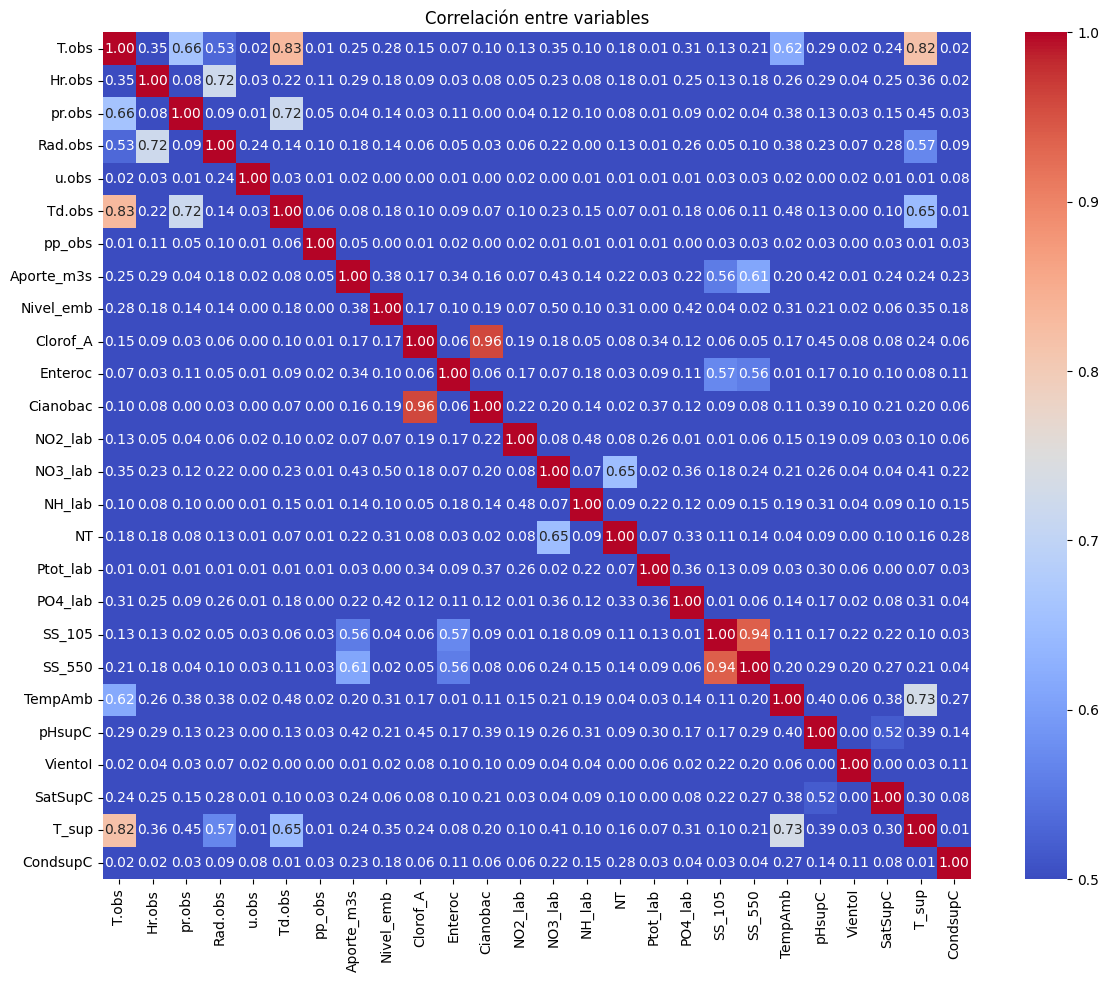
\includegraphics[width=0.90\textwidth]{Imagenes/Correlacion_Heatmap.png}
    \caption{Matriz de correlación entre variables (coeficientes > 0.5).}
    \label{fig:correlaciones}
\end{figure}

\subsection{Relación de variables con el nivel de alerta}

Se evaluó la dependencia entre cada variable y el nivel de alerta (\texttt{Target}) utilizando la métrica de información mutua, que permite capturar tanto relaciones lineales como no lineales entre variables.

Los resultados (ver Figura~\ref{fig:mutual-info}) indican que las variables más informativas para la clasificación del nivel de alerta son:

\begin{itemize}
  \item \textbf{Cianobac} y \textbf{Clorof\_A}: indicadores directos de la biomasa fitoplanctónica y la presencia de cianobacterias, fuertemente asociados a episodios de riesgo.
  
  \item \textbf{NO3\_lab}, \textbf{Ptot\_lab} y \textbf{SS\_105}: representan condiciones de eutrofización (exceso de nutrientes), que favorecen el desarrollo de floraciones algales.
  
  \item \textbf{NO2\_lab}, \textbf{NH\_lab} y \textbf{SS\_550}: reflejan procesos de descomposición y transformación del nitrógeno, así como la carga particulada en capas más profundas del cuerpo de agua.
\end{itemize}


Las variables meteorológicas (\texttt{Rad.obs}, \texttt{pr.obs}, \texttt{Hr.obs}, etc.) aportan menor información individual, aunque pueden tener valor complementario al combinarse con variables biológicas e hidrológicas.

\begin{figure}[H]
    \centering
    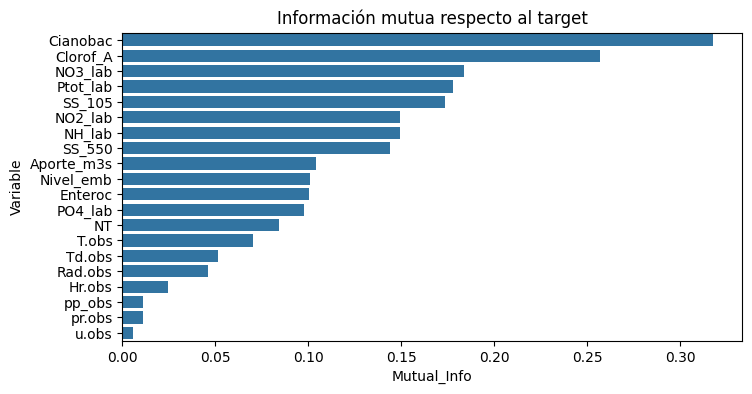
\includegraphics[width=0.85\textwidth]{Imagenes/Mutual_Info_Target.png}
    \caption{Ranking de variables según su información mutua con respecto al nivel de alerta.}
    \label{fig:mutual-info}
\end{figure}


\subsection{Patrones temporales}

Se graficaron las series temporales suavizadas (media móvil de 7 días) de cuatro variables claves: \texttt{Cianobac}, \texttt{Clorof\_A}, \texttt{Aporte\_m3s} y \texttt{T.obs}. La Figura~\ref{fig:series-temporales} muestra su evolución a lo largo del período 2020–2025.

El caudal de aporte (\texttt{Aporte\_m3s}) exhibe un patrón estacional con bajas precipitaciones en verano donde la temperatura del agua (\texttt{T.obs}) sigue un ciclo anual regular, con máximos en verano y mínimos en invierno, patrón consistente con la estacionalidad esperada en la región.

\begin{figure}[H]
    \centering
    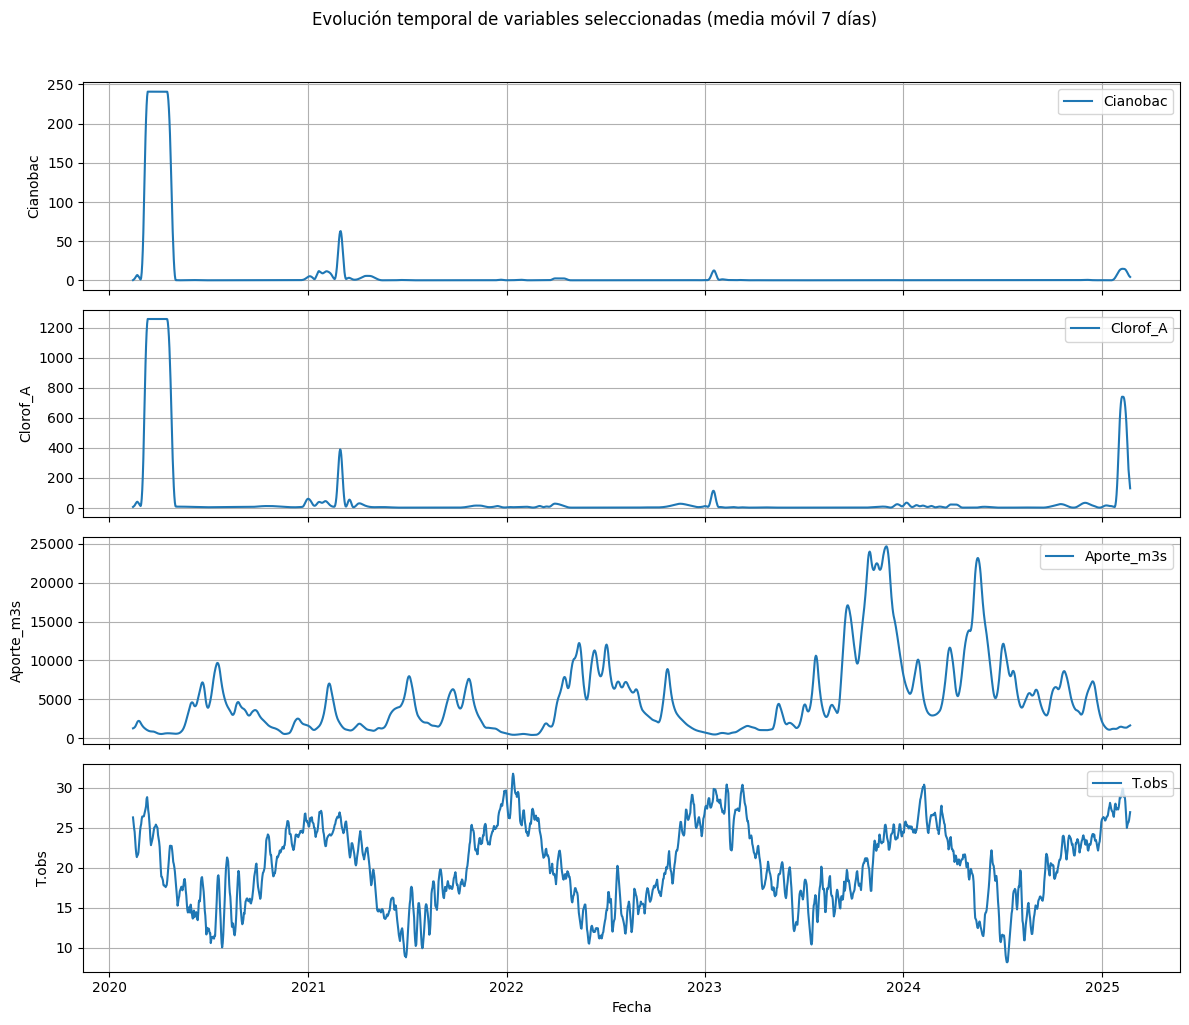
\includegraphics[width=0.95\textwidth]{Imagenes/Series_Temporales.png}
    \caption{Evolución temporal de variables seleccionadas (media móvil de 7 días). Se observan eventos de floración mas marcados en los veranos de 2020, 2021, 2023 y 2025.}
    \label{fig:series-temporales}
\end{figure}

\subsection{Distribución de clases en la variable objetivo}

La Figura~\ref{fig:distribucion-clases} muestra la distribución de clases en la variable objetivo utilizada para la predicción del nivel de alerta. Se observa un fuerte desbalance de clases, con una gran mayoría de observaciones correspondientes a la clase \textbf{0.0} (estado sin riesgo), que representa aproximadamente el 80\% del total. Las clases 1.0, 2.0 y 3.0, que indican niveles crecientes de alerta sanitaria, están considerablemente subrepresentadas, especialmente la clase 2.0.

Este desbalance plantea un desafío importante para los modelos de clasificación, ya que puede llevar a un sesgo hacia la clase mayoritaria y una baja sensibilidad frente a situaciones críticas.

\begin{figure}[H]
\centering
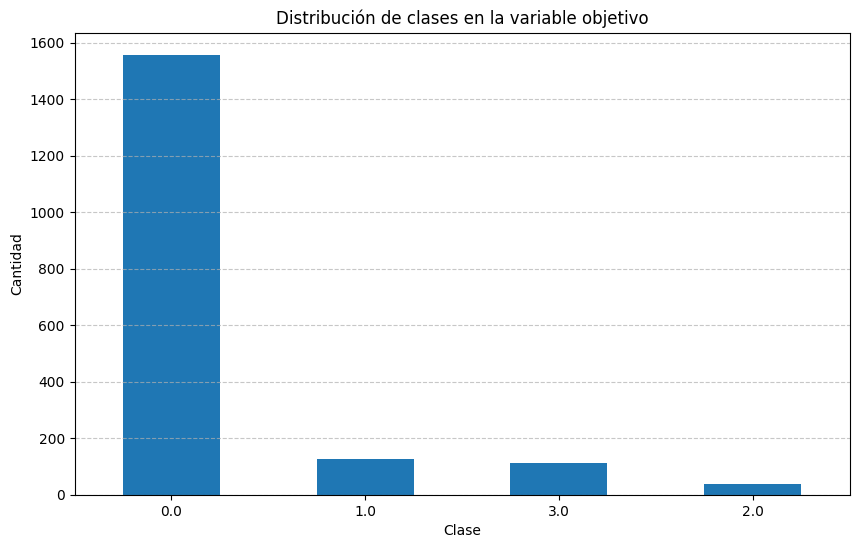
\includegraphics[width=0.7\textwidth]{Imagenes/Distribucion_clases.png}
\caption{Distribución de clases en la variable objetivo}
\label{fig:distribucion-clases}
\end{figure}


%###################################################################################################

\section{Descripción de las técnicas de análisis y modelado}

\subsection{Validación y búsqueda de hiperparámetros con Walk-Forward}

Con el objetivo de seleccionar los mejores hiperparámetros para los modelos predictivos utilizados, se implementó una estrategia de validación basada en la técnica Walk-Forward, la cual permite una evaluación realista del desempeño del modelo en un contexto temporal.

\textbf{Búsqueda de hiperparámetros.}

Para cada combinación de hiperparámetros, se realizó una serie de 60 entrenamientos consecutivos. En cada iteración:

Se utilizó una ventana de entrenamiento desde el inicio del data set hasta el inicio del conjunto de validación.

Se entrenó el modelo y se realizó la predicción del día siguiente, el primero de los 60 reservados para validación.

El día predicho se incorporó al conjunto de entrenamiento, desplazando la ventana una unidad hacia adelante (rolling window).

Este procedimiento se repitió hasta completar la predicción de 60 días consecutivos. La métrica utilizada para comparar combinaciones de hiperparámetros fue el accuracy obtenido en esas 60 predicciones.

\textbf{Evaluación final con conjunto de prueba.}

Una vez seleccionada la mejor configuración de hiperparámetros, se aplicó la misma técnica de Walk-Forward sobre un conjunto de 30 días reservados para prueba. 
Para ello:
Se utilizaron todos los registros anteriores como conjunto de entrenamiento inicial.
Se aplicó nuevamente el esquema secuencial de entrenamiento y prueba diario, conservando el orden temporal.

Esta evaluación final permitió estimar el desempeño real del modelo con los hiperparámetros seleccionados, evitando cualquier tipo de fuga de información.

Esta metodología asegura una validación robusta y temporalmente coherente, adecuada para tareas de predicción sobre series cronológicas, como lo es la calidad del agua.\cite{brownlee2018walkforward}

\section{Descripción de la selección de características}

\textbf{Transformación de la variable temporal.}

La variable temporal original, representada como fechas, fue transformada a valores enteros utilizando como referencia el 1 de enero de 1900. Esta conversión garantiza la continuidad y secuencia de los datos, facilitando su procesamiento por los modelos de aprendizaje automático. Es importante destacar que la división entre los conjuntos de entrenamiento y prueba se realizó antes de esta transformación.


\subsection{Selección de características}

Para el modelo de \textbf{Random Forest}, se consideraron inicialmente todas las características disponibles, aprovechando su capacidad para manejar conjuntos de datos con múltiples variables y evaluar la importancia de cada una en la predicción. A partir de los resultados de importancia, se seleccionó un subconjunto de variables cuya contribución superaba el \textbf{2\%} en la métrica de importancia relativa. Este conjunto reducido fue utilizado en las pruebas con \textbf{Regresión Logística Multinomial (RL)} y \textbf{Máquinas de Vectores de Soporte (SVM)}, con el fin de reducir la dimensionalidad y mejorar la eficiencia computacional.

En el caso del modelo \textbf{LightGBM}, se volvió a utilizar el conjunto completo de variables, dada su eficiencia para procesar grandes volúmenes de atributos y realizar selección interna de características durante el entrenamiento.


\section{Descripción de las métricas de evaluación}


%-------------------------------------------------------------
\subsection{Métricas de evaluación}
%-------------------------------------------------------------
Los modelos se compararán utilizando métricas recomendadas para problemas
multiclase y con fuerte desbalance en la variable objetivo \citep{Powers2011}:

\begin{itemize}[noitemsep]
  \item \textbf{F1–score macro}\,: media armónica entre precisión y \textit{recall} por clase, otorga igual peso a cada clase independientemente de su frecuencia.
  \item \textbf{Recall por clase}\,: permite evaluar qué tan bien el modelo identifica correctamente las instancias verdaderas de cada categoría, lo cual es clave en contextos donde los estados críticos están subrepresentados.
\end{itemize}

Se enfatiza el análisis de las \textbf{matrices de confusión} para test, lo cual permite observar explícitamente los aciertos y errores en la clasificación de cada clase.



\section{Descripción de los métodos de Machine Learning}

Se evaluarán cuatro algoritmos supervisados multiclase:

\begin{enumerate}[noitemsep]
\item \textbf{Regresión logística multinomial}\,: modelo lineal que
      estima las probabilidades de pertenencia a cada nivel mediante
      la función \textit{softmax}. Ofrece interpretabilidad de
      coeficientes.
\item \textbf{Máquinas de Soporte Vectorial (MSV)}\,: se utilizaran dos nucleos Linear y RBF para capturar relaciones no lineales.
\item \textbf{Random Forest}\,: ensamble de árboles de decisión, robusto a ruido y que maneja interacciones
      variable–variable de forma automática.
\item \textbf{Light Gradient Boosting Machine (LGBM)}\,: algoritmo
      \emph{boosting} basado en histogramas, adecuado para datos heterogéneos y de gran tamaño.
\end{enumerate}

%-------------------------------------------------------------
\chapter{Resultados y discusión}
%-------------------------------------------------------------
\section{Presentación y análisis de resultados obtenidos}

En esta sección se presentan los resultados obtenidos tras el entrenamiento de los modelos de Machine Learning propuestos. Cada subsección detalla el desempeño individual del modelo, sus principales métricas, y observaciones sobre su comportamiento frente al conjunto de test.

\subsection{Random Forest}

El modelo de \textit{Random Forest} fue entrenado utilizando una búsqueda en malla (\textit{Grid Search}) sobre los siguientes hiperparámetros:

\begin{itemize}[noitemsep]
  \item \texttt{n\_estimators}: \{50, 100, 200, 300, 400\}
  \item \texttt{max\_depth}: \{2, 3, 5, 10, None\}
  \item \texttt{min\_samples\_split}: \{2, 3, 5\}
  \item \texttt{min\_samples\_leaf}: \{1, 2, 3\}
\end{itemize}

Los mejores hiperparámetros encontrados fueron:
\begin{center}
\texttt{\{'n\_estimators': 200, 'max\_depth': None, 'min\_samples\_split': 2, 'min\_samples\_leaf': 1\}}
\end{center}

El modelo alcanzó una exactitud del \textbf{0.9167} sobre el conjunto de validación. En cuanto a la evaluación en test logró una exactitud del \textbf{0.9333} y F1-score (macro): 0.9491.  
A continuación se presenta la matriz de confusión correspondiente al conjunto de test:

\begin{figure}[H]
    \centering
    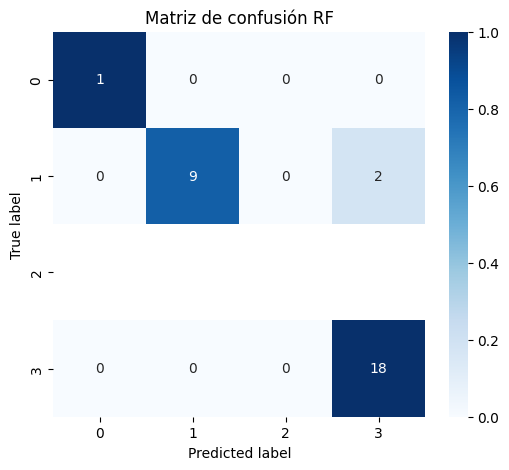
\includegraphics[width=0.55\textwidth]{Imagenes/Matriz-Randomforest.png}
    \caption{Matriz de confusión para el modelo Random Forest.}
    \label{fig:cm-randomforest}
\end{figure}

\begin{table}[H]
\centering
\caption{Recall por clase en el modelo Random Forest}
\label{tab:recall-rf}
\begin{tabular}{lcc}
\toprule
\textbf{Clase} & \textbf{Descripción} & \textbf{Recall} \\
\midrule
0 & Sin alerta           & 1.00 \\
1 & Alerta 0          & 0.82 \\
2 & Alerta 1         & -- \\
3 & Alerta 2 (crítica) & 1.00 \\
\bottomrule
\end{tabular}
\end{table}

La matriz de confusión (ver Figura~\ref{fig:cm-randomforest}) muestra que el modelo logra identificar con alta precisión las clases extremas: la clase 0 (sin alerta) y la clase 3 (Alerta 2), ambas con un recall de 1.0. La clase 1 presenta un rendimiento levemente inferior (recall $\approx 0.82$), con algunos errores de clasificación hacia la clase 3. No se registran observaciones reales de la clase 2 en este conjunto de test, por lo que no se puede calcular su recall. Los valores de \textit{recall} por clase se resumen en la Tabla~\ref{tab:recall-rf}. El comportamiento del modelo sugiere buena capacidad para distinguir entre estados contrastantes, aunque podrían requerirse más observaciones en clases intermedias para fortalecer la generalización en situaciones transicionales.

\textbf{Importancia de variables en Random Forest.}

\begin{figure}[H]
    \centering
    \includegraphics[width=\textwidth]{Imagenes/importancia_rf.png}
    \caption{Importancia promedio de atributos de todas las iteraciones del modelo Random Forest.}
    \label{fig:importancia-rf}
\end{figure}

Como se observa en la Figura~\ref{fig:importancia-rf}, las variables \texttt{Cianobac}, \texttt{MicrtEli}, \texttt{time{\_}int}  y \texttt{Clorof{\_}A} resultaron ser las más relevantes en la predicción del estado de alerta, seguidas por parámetros relacionados con nutrientes como \texttt{Ptot{\_}lab}, \texttt{NH{\_}lab} y otras con niveles significantes. También se destacan variables físico-químicas como \texttt{pHsupC}, \texttt{TursupC} y  \texttt{SS{\_}105} lo cual refuerza la influencia de condiciones biológicas y de turbidez en la clasificación. Las variables meteorológicas pronosticadas, en cambio, aportan menor valor predictivo en este modelo.

\subsection{LightGBM}

El modelo \textit{LightGBM} fue entrenado utilizando una optimización bayesiana con \textit{Optuna}, explorando el siguiente espacio de hiperparámetros:

\begin{itemize}[noitemsep]
  \item \texttt{learning\_rate}: \{0.01, 0.05, 0.1\}
  \item \texttt{n\_estimators}: \{100, 200\}
  \item \texttt{max\_depth}: \{3, 5, 7\}
  \item \texttt{num\_leaves}: \{31, 63, 127\}
  \item \texttt{min\_child\_samples}: \{20, 50\}
  \item \texttt{subsample}, \texttt{colsample\_bytree}: \{0.8, 1.0\}
  \item \texttt{reg\_alpha}, \texttt{reg\_lambda}: \{0, 0.1\}
\end{itemize}

Los mejores hiperparámetros encontrados fueron:
\begin{center}
\texttt{\{objective=multiclass, metric=multi\_logloss, learning\_rate=0.0445, n\_estimators=118,} \\
\texttt{max\_depth=7, num\_leaves=64, min\_child\_samples=67, subsample=0.671,} \\
\texttt{colsample\_bytree=0.607, reg\_alpha=7.18e-4, reg\_lambda=3.24e-4\}}
\end{center}

El modelo alcanzó una exactitud promedio de \textbf{0.9333} durante la validación. En el conjunto de test se obtuvo una exactitud de \textbf{0.9000} y un F1-score macro de \textbf{0.8285}.  
A continuación se presenta la matriz de confusión correspondiente:

\begin{figure}[H]
    \centering
    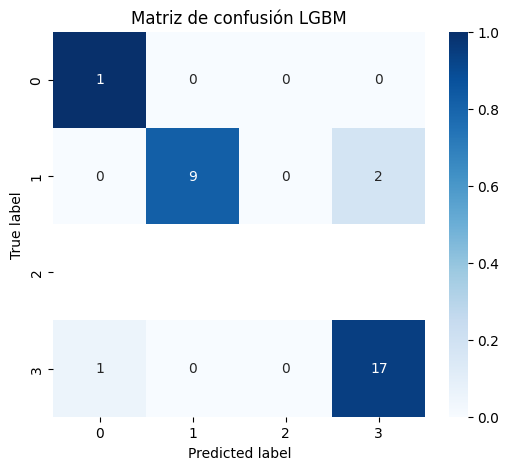
\includegraphics[width=0.55\textwidth]{Imagenes/Matriz_LGBM_Test.png}
    \caption{Matriz de confusión para el modelo LightGBM.}
    \label{fig:cm-lgbm}
\end{figure}

\begin{table}[H]
\centering
\caption{Recall por clase en el modelo LightGBM}
\label{tab:recall-lgbm}
\begin{tabular}{lcc}
\toprule
\textbf{Clase} & \textbf{Descripción} & \textbf{Recall} \\
\midrule
0 & Sin alerta           & 1.00 \\
1 & Alerta 0             & 0.82 \\
2 & Alerta 1             & -- \\
3 & Alerta 2 (crítica)   & 0.94 \\
\bottomrule
\end{tabular}
\end{table}

La matriz de confusión (ver Figura~\ref{fig:cm-lgbm}) muestra que el modelo logra clasificar correctamente la mayoría de las instancias de clase 3 (Alerta 2), aunque con un leve descenso en el recall respecto a Random Forest (recall = 0.94). También se observa una clasificación correcta de la clase 0 (sin alerta), mientras que la clase 1 mantiene un rendimiento similar (recall $\approx 0.82$). No se registraron observaciones de la clase 2 en este conjunto de test. Los valores de \textit{recall} por clase se resumen en la Tabla~\ref{tab:recall-lgbm}. En conjunto, el modelo demuestra buena capacidad discriminativa, con un balance razonable entre precisión y sensibilidad, aunque con una leve pérdida de robustez en los extremos críticos.


\subsection{Otros modelos evaluados}

Además de los modelos presentados, se realizaron pruebas con \textbf{Regresión Logística Multinomial} y \textbf{Máquinas de Soporte Vectorial (MSV)} utilizando el conjunto reducido de variables seleccionadas por importancia. Sin embargo, ambos modelos presentaron un desempeño muy pobre en comparación con Random Forest y LightGBM.

\begin{itemize}[noitemsep]
  \item \textbf{Regresión Logística:} Exactitud: 0.3000, F1-score macro: 0.2059
  \item \textbf{SVM:} Exactitud: 0.2000, F1-score macro: 0.2000
\end{itemize}

Estos resultados indican una baja capacidad de generalización, posiblemente asociada a la naturaleza del problema, el desbalance de clases y la limitada expresividad de estos modelos en este contexto.


\subsection{Discusión de los resultados y su relevancia}

Los resultados obtenidos muestran un desempeño destacado de los modelos \textit{Random Forest} y \textit{LightGBM}, que alcanzaron valores de exactitud superiores al 90\% y F1-score macro por encima de 0.82 en los conjuntos de test. Estas métricas superan ampliamente a las obtenidas por modelos lineales como la regresión logística o SVM, confirmando la superioridad de enfoques no lineales para este tipo de tareas. Este comportamiento es coherente con hallazgos previos en la literatura, donde modelos de árboles también se destacaron en la predicción de variables como clorofila-\emph{a} o calidad de agua en lagos del hemisferio sur \citep{RodriguezLopez2023}, así como en revisiones generales sobre el uso de aprendizaje automático en sistemas acuáticos \citep{Schaeffer2024}.

Desde una perspectiva ambiental, estos modelos demostraron capacidad para identificar correctamente los estados más críticos de calidad del agua (clase 3), lo cual representa una contribución relevante para sistemas de alerta temprana. La alta tasa de aciertos en estas clases sugiere que los modelos pueden ser herramientas útiles en la gestión del riesgo sanitario y recreativo en cuerpos de agua como el embalse de Salto Grande.

En cuanto a las variables más relevantes para la predicción, los resultados reflejan una clara preponderancia de indicadores biológicos y fisicoquímicos, \texttt{Cianobac}, \texttt{MicrtEli}, \texttt{Ptot\_lab}, \texttt{NT}, \texttt{Clorof\_A}, por sobre las variables meteorológicas o pronosticadas. Esta observación es consistente con estudios que destacan el rol predominante de los nutrientes (N, P) como impulsores del crecimiento de cianobacterias, por encima de factores climáticos como la temperatura, particularmente en cuerpos de agua continentales templados \citep{Rigosi2014}.

Finalmente, la implementación de modelos de aprendizaje automático no lineales permitió abordar la complejidad inherente a la dinámica ecológica del embalse, compensando parcialmente las limitaciones asociadas a la escasez y dispersión temporal de los datos disponibles. Esta evidencia refuerza el potencial de estas herramientas para su integración en esquemas de monitoreo ambiental y evaluación predictiva localizada.

\subsection{Limitaciones y posibles mejoras}

A pesar de los resultados prometedores obtenidos, el estudio presenta una serie de limitaciones tanto a nivel de datos como de enfoque metodológico, que deben ser consideradas al interpretar los hallazgos y planificar desarrollos futuros.

En primer lugar, el desbalance en la variable objetivo constituye un desafío relevante: la clase 0 (sin alerta) domina ampliamente el conjunto de datos, mientras que las clases correspondientes a niveles de riesgo medio o alto están subrepresentadas. Esto limita la capacidad del modelo para aprender patrones asociados a eventos críticos. Además, la cantidad limitada de observaciones reales restringe el entrenamiento de modelos más complejos o sensibles a la varianza. La frecuencia irregular de muestreo, semanal en verano y mensual en invierno, también dificulta la modelización temporal. Por otro lado, debido a la partición de test generada mediante la técnica \textit{walk-forward}, ciertas clases no están representadas, lo que impide calcular métricas como el \textit{recall} para cada clase.


A esto se suma que, debido a la falta de continuidad en las observaciones, no fue posible construir un conjunto de entrenamiento totalmente real que permitiera comparar de forma controlada el desempeño del modelo con y sin interpolación. Esta limitación impide cuantificar el impacto exacto de los datos sintéticos y representa un aspecto clave a explorar en trabajos futuros.

Desde el punto de vista metodológico, no se incorporaron enfoques explícitos de modelado de series temporales, como \textit{Long Short-Term Memory (LSTM)} o \textit{Prophet}, que podrían capturar patrones secuenciales o estacionales relevantes en la dinámica ecológica del sistema.

Si bien la interpolación de variables clave fue necesaria para compensar la escasez y dispersión temporal de los datos, en especial para atributos biológicos, esta estrategia introduce un riesgo potencial de sobreajuste. El modelo podría aprender patrones artificiales generados por la interpolación, en lugar de relaciones efectivamente observadas en el sistema. No obstante, esta técnica resultó indispensable para mantener un volumen suficiente de datos de entrenamiento. Sería deseable en futuros estudios evaluar formalmente el impacto de los datos sintéticos, comparando el desempeño del modelo con y sin interpolación, preferentemente sobre conjuntos de test construidos exclusivamente a partir de registros reales.

Como líneas de mejora, se propone ampliar el dataset mediante la incorporación de campañas históricas y datos de estaciones ubicadas en otros puntos del lago. También se recomienda evaluar el desempeño de modelos probabilísticos o híbridos, que integren la predicción con la estimación de incertidumbre. Finalmente, sería conveniente implementar esquemas de validación empleando años completamente excluidos del entrenamiento, ya que esto permitiría evaluar con mayor realismo la capacidad de generalización de los modelos desarrollados.

%-------------------------------------------------------------
\chapter{Conclusión}
%-------------------------------------------------------------

\section{Resumen de los hallazgos principales}

Se desarrollaron modelos de predicción de calidad del agua con horizonte semanal, aplicados al embalse de Salto Grande, integrando datos satelitales, in situ, meteorológicos e hidrológicos. Entre los algoritmos evaluados, \textbf{Random Forest} y \textbf{LightGBM} demostraron un desempeño robusto, alcanzando exactitudes superiores al 90\% y F1-score macro por encima de 0.82. Estos modelos lograron identificar correctamente los estados críticos de alerta, con un alto recall en la clase de mayor riesgo. Las variables biológicas y fisicoquímicas, en especial cianobacterias, clorofila y nutrientes, resultaron ser las más relevantes para la predicción.

\section{Conclusiones generales y relación con los objetivos}

El estudio confirma la factibilidad de proyectar el estado de calidad del agua con hasta 7 días de anticipación en condiciones reales de monitoreo, utilizando técnicas de Machine Learning. Los resultados permiten afirmar que estas herramientas pueden ser integradas a esquemas de alerta temprana, fortaleciendo la toma de decisiones para el uso recreativo y sanitario del recurso en playas específicas como Las Palmeras. Se logró así responder positivamente a la pregunta planteada y cumplir con el objetivo general del trabajo.

\section{Recomendaciones para futuros trabajos}

Se recomienda ampliar el volumen y la cobertura temporal del conjunto de datos, así como incorporar nuevas fuentes satelitales, posiblemente mediante la contratación de servicios complementarios a los actualmente utilizados, con el objetivo de mejorar la resolución y frecuencia de observación. También se sugiere implementar modelos secuenciales que capten mejor la dinámica temporal de las variables, y evaluar la transferencia del enfoque desarrollado a otras estaciones del embalse, mediante un entrenamiento conjunto o comparativo entre sitios.

Una línea de trabajo futura relevante consiste en explorar horizontes de predicción más amplios, por ejemplo, extendiendo la proyección a 14 días. La elección del horizonte de 7 días en este estudio respondió a una necesidad operativa concreta: generar informes semanales de calidad del agua, solicitados por el organismo responsable durante la temporada de mayor uso recreativo (noviembre a marzo). Esta ventana representa un compromiso entre utilidad práctica y estabilidad predictiva, ya que la variabilidad de nutrientes y la incertidumbre en los pronósticos meteorológicos aumentan considerablemente a medida que se extiende el plazo.

No obstante, evaluar horizontes más largos permitiría anticipar eventos críticos con mayor antelación, lo cual resulta especialmente valioso en contextos de alerta sanitaria o planificación preventiva. Asimismo, se propone analizar más detalladamente los días intermedios entre el estado actual y la predicción a 7 días, particularmente en aquellos casos donde se produce un cambio de clase. Esta estrategia permitiría identificar el momento probable del quiebre y profundizar en el análisis de las variables que lo anticipan, aportando evidencia adicional sobre los atributos más determinantes en la dinámica transicional de la calidad del agua.


% Capítulo 6: Bibliografía
\cleardoublepage
\bibliographystyle{apacite}
\bibliography{references}




% Capítulo 7: Anexos
\appendix
\chapter{Anexos}
\section{Repositorio en GitHub}

https://github.com/JoacoTschopp?tab=repositories

\end{document}






%######################
-El trabajo se encuentra muy bien planteado, tanto a nivel conceptual como metodológico. 

-Sólo algunas sugerencias:

-Sería bueno incorporar una medida de cómo afecta al modelo  la inclusión de datos sintéticos, discutiendo potencial riesgo de sobreajuste.

-Discutir la posibilidad de extender el horizonte de predicción más allá de 7 días.